\documentclass[../thesis.tex]{subfiles}

\begin{document}

\chapter{The Daya Bay experiment}
\label{chap:experim}

\section*{Introduction}

The Daya Bay experiment was designed to measure $\theta_{13}$ by observing the antineutrinos produced by the six 2.9~GW$_{\text{th}}$ nuclear reactors of the Daya Bay and Ling Ao power plants, located near Shenzhen in southern China. A total of eight functionally identical antineutrino detectors (ADs) were deployed, each containing a target of 20~tons of gadolinium-doped liquid scintillator (GdLS). Four of the ADs were evenly divided among two near halls ($\sim$350-600~m baselines from the cores), and the remaining four were placed in a single far hall ($\sim$1500-1950~m baselines). Shielding from cosmic rays was provided by $\sim$100~m and $\sim$300~m, respectively, of mountainous overburden at the near and far halls. The ADs in each hall were immersed in instrumented water pools which provided shielding from ambient radioactivity and detection of Cerenkov radiation from atmospheric muons. Redundant detection of muons, as well as directional information, were made available by resistive plate chambers (RPCs) laid on top of the water pools. In this chapter we discuss further details of the layout, the detectors, and the shielding and vetoing system of the experiment.

\section{Site layout}
\label{sec:expLayout}

\begin{figure}[ht]
  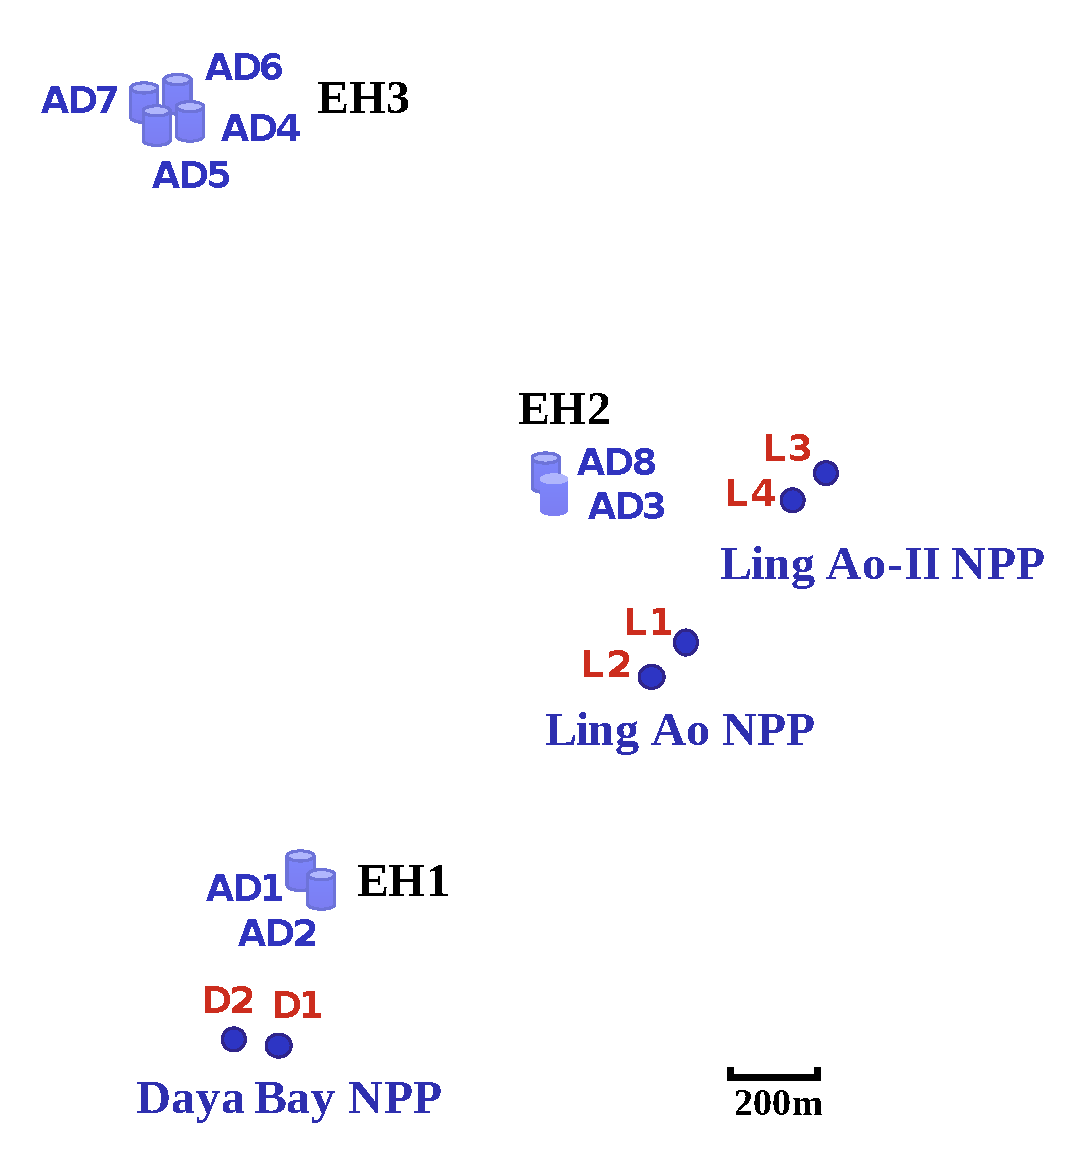
\includegraphics[scale=0.4]{inkLayout.pdf}
  \caption{The layout of the Daya Bay experiment. Modified from \cite{SideBySide}.}
  \label{fig:layout} 
\end{figure}

As shown in \autoref{fig:layout}, the power reactors are divided into three nuclear power plants (NPPs) of two cores each. One of the two clusters contains the Daya Bay NPP (cores D1 and D2), while the other cluster consists of the Ling Ao (L1 and L2) and Ling Ao-II (L3 and L4) NPPs. EH1 is located around 350~m from the Daya Bay NPP, while EH2 is roughly 500~m from the two Ling Ao NPPs. The far hall, EH3, in turn is located about 1900~m from the Daya Bay NPP and 1500~m from the Ling Ao NPPs. The measured baselines, as determined from a combined GPS and total station theodolite survey, are given in \autoref{tab:expBaselines}. The uncertainty of $\sim$2~cm in these measurements was shown to have negligible impact on the analysis; likewise, reactor simulations determined that the centroid of $\nubar_e$ emission to be within $\sim$2~cm of each core's center. Although $\nubar_e$ emission was distributed across the $\sim$3~m-scale volume of each core, the analysis treats each core as a point source, given that these geometric effects are negligible at Daya Bay's baselines.

\begin{table}[ht]
  \begin{tabular}{lcrrrrrr}
    \toprule
    \multicolumn{2}{c}{} & \multicolumn{6}{c}{Reactor baseline [m]} \\
    \cmidrule{3-8}
    Hall & Detector & \multicolumn{1}{c}{D1} & \multicolumn{1}{c}{D2} & \multicolumn{1}{c}{L1} & \multicolumn{1}{c}{L2} & \multicolumn{1}{c}{L3} & \multicolumn{1}{c}{L4} \\
    \midrule
    EH1  & AD1      & 362.38  & 371.76  & 903.47  & 817.16  & 1353.62 & 1265.32 \\
         & AD2      & 357.94  & 368.41  & 903.35  & 816.90  & 1354.23 & 1265.89 \\
    EH2  & AD3      & 1332.48 & 1358.15 & 467.57  & 489.58  & 557.58  & 499.21  \\
         & AD8      & 1337.43 & 1362.88 & 472.97  & 495.35  & 558.71  & 501.07  \\
    EH3  & AD4      & 1919.63 & 1894.34 & 1533.18 & 1533.63 & 1551.38 & 1524.94 \\
         & AD5      & 1917.52 & 1891.98 & 1534.92 & 1535.03 & 1554.77 & 1528.05 \\
         & AD6      & 1925.26 & 1899.86 & 1538.93 & 1539.47 & 1556.34 & 1530.08 \\
         & AD7      & 1923.15 & 1897.51 & 1540.67 & 1540.87 & 1559.72 & 1533.18 \\
    \bottomrule
    % \multirow{2}{*}{EH1} & AD1      & 362.38  & 371.76  & 903.47  & 817.16  & 1353.62 & 1265.32 \\
  \end{tabular}
  \caption{Baselines between geometric centers of the ADs and of the reactor cores. From \cite{An_2017}.}
  \label{tab:expBaselines}
\end{table}

\section{Antineutrino detectors}
\label{sec:expADs}

\begin{figure}[ht]
  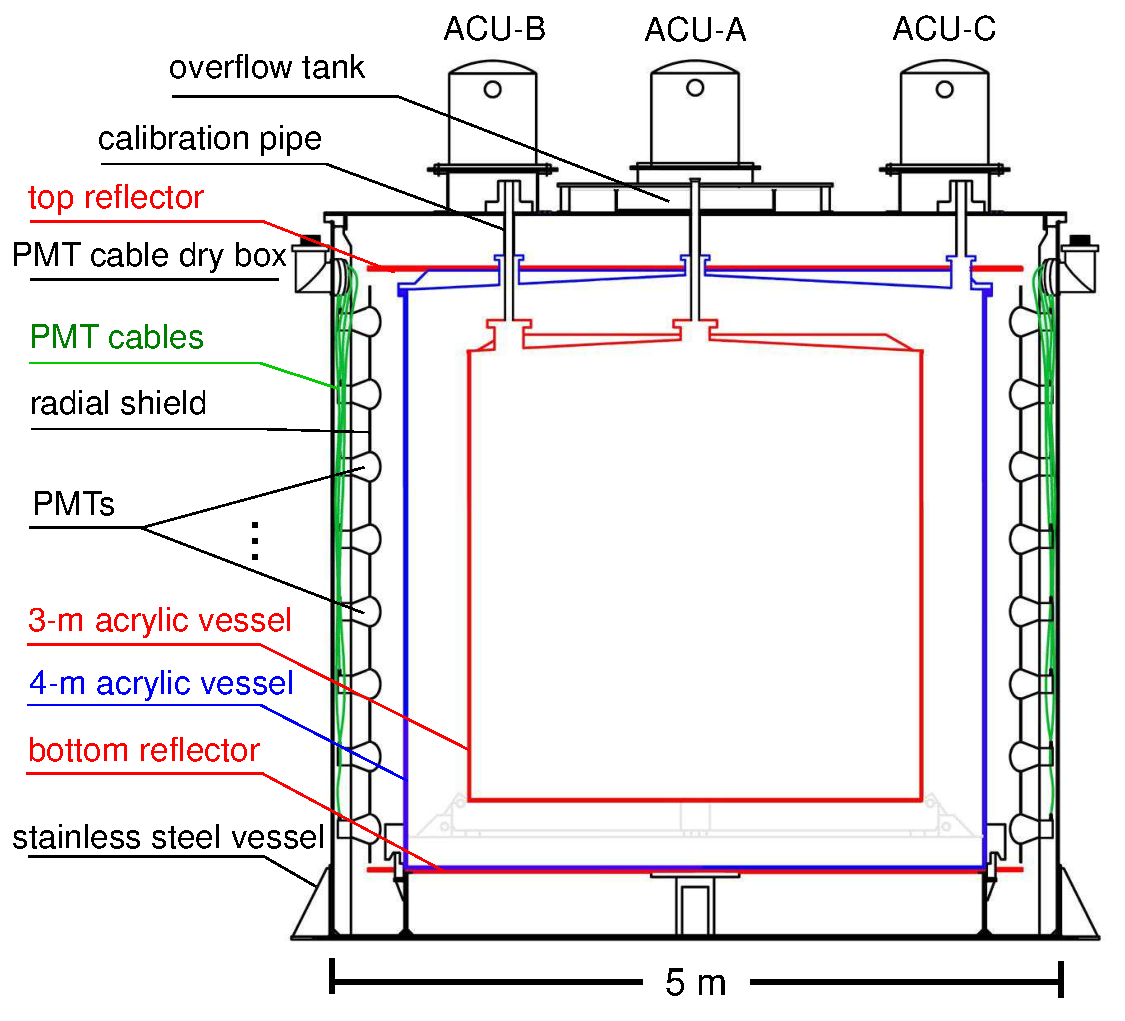
\includegraphics[scale=0.4]{exp_AD_structure.pdf}
  \caption{Structure of a Daya Bay antineutrino detector. From \cite{An_2017}.}
  \label{fig:expDetector}
\end{figure}

The design of the Daya Bay ADs is shown in \autoref{fig:expDetector}. Each AD is made of a cylindrical stainless steel vessel (SSV), $\sim$5~m in diameter and height, containing two nested cylinders of UV-transparent acrylic. The 3m-square inner acrylic vessel (IAV) contains the target mass of 20~t of GdLS\footnote{Daya Bay's liquid scintillator consists of linear alkyl benzene (LAB) as the solvent and medium, 3~g/L of 2,5-diphenyloxazole (PPO) as the fluor, and 15~mg/L of p-bis-(o-methystyril)-benzene (bis-MSB) as the wavelength shifter. For the GdLS, 0.1\% $^{\text{nat}}$Gd by mass was added in the form of a complex with 3,5,5-trimethylhexanoic acid (THMA). Further details can be found in \cite{Beriguete_2014}.}. Surrounding it is the 4m-square outer acrylic vessel (OAV), which contains 20~t of \emph{Gd-free} LS. This ``gamma catcher'' volume ensures the full containment and measurement of gammas produced near the edge of the GdLS, while also providing additional target mass for studies that use neutron capture on hydrogen instead of on gadolinium. Between the OAV and the inner wall of the SSV, a 37~t volume of transparent mineral oil (MO) provides shielding from radioactivity in the detector materials, in addition to its role in balancing the stress on the OAV wall.

Within the MO volume, the inner sidewall of the SSV supports 192 8-inch Hamamatsu R5912 photomultipler tubes (PMTs) to detect the light from scintillation. The PMTs are arranged in eight rings of 24 tubes whose photocathodes protrude from matte-black radial shields that fully cover the sidewalls, preventing light from reflecting off the walls. This simplifies the optical characteristics of the ADs, reducing the complexity of vertex reconstruction. Conversely, however, reflective discs are installed at the top and bottom of the AD, improving the uniformity of light collection versus event position. Each PMT is outfitted with a FINEMET conical magnetic shield to minimize azimuthal variations in PMT response caused by the Earth's magentic field.

\subsection{Detection principle}
\label{sec:expDetPrinc}

\begin{figure}[ht]
  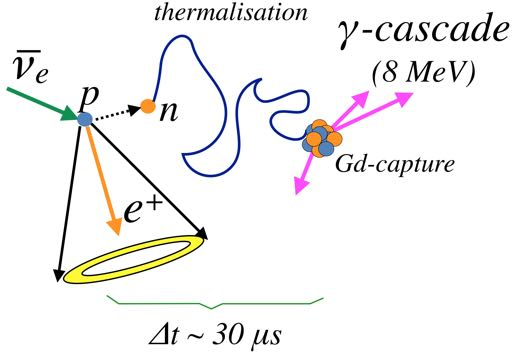
\includegraphics[scale=0.4]{ibd.png}
  \caption{An illustration of the inverse beta decay reaction. Unlike a water Cerenkov detector, a Daya Bay AD cannot discern the direction of the positron. From \cite{Fernandez_2017}.}
  \label{fig:expIBD}
\end{figure}

\section{Shielding/vetoing system}
\label{sec:expShieldVeto}

\begin{figure}[ht]
  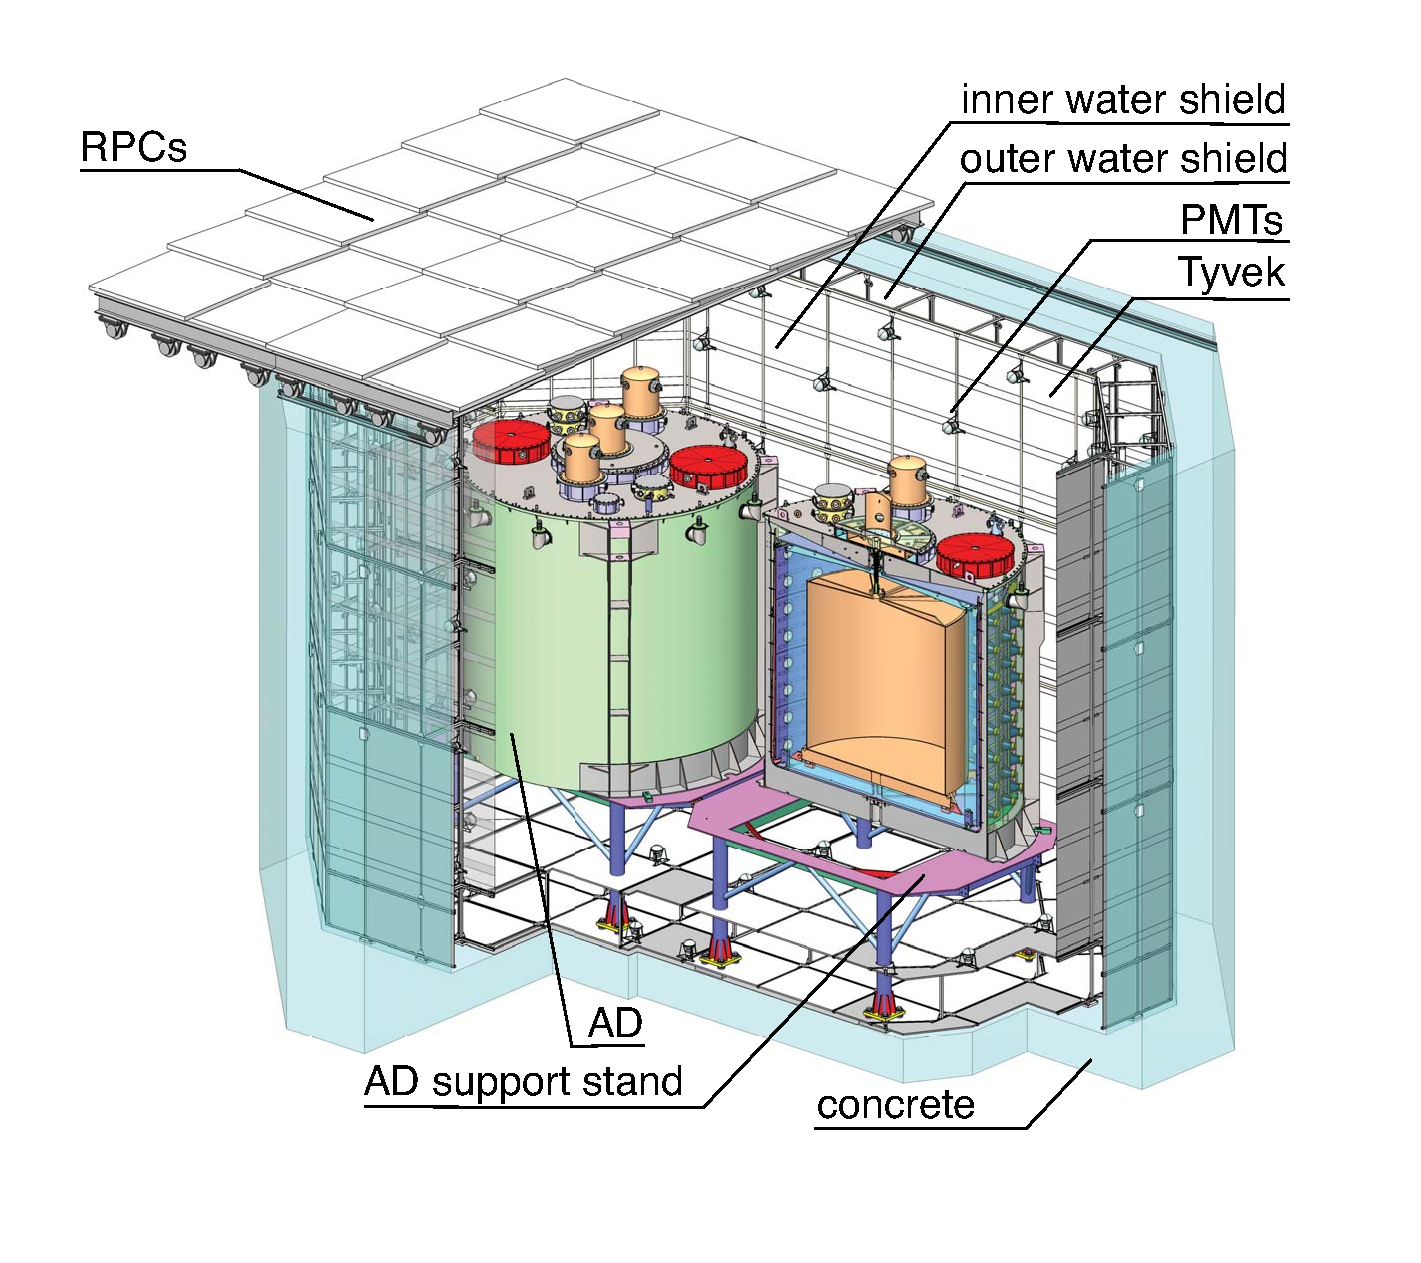
\includegraphics[scale=0.4]{exp_near_site_diagram.pdf}
  \caption{Water pool (including ADs) as configured in the near halls. The far hall is similar, with four ADs instead of two. From \cite{An_2017}.}
  \label{fig:expPool}
\end{figure}

\subfilebackmatter

\end{document}